\documentclass{article}
\usepackage[preprint]{neurips_2026}

\usepackage[utf8]{inputenc}
\usepackage[T1]{fontenc}
\usepackage{hyperref}
\usepackage{url}
\usepackage{booktabs}
\usepackage{amsfonts}
\usepackage{amsmath}
\usepackage{amssymb}
\usepackage{graphicx}
\usepackage{xcolor}
\usepackage{algorithm}
\usepackage{algpseudocode}
\usepackage{multirow}
\usepackage{array}
\usepackage{caption}

\title{Cognitive State Compilation: Resource-Bounded Construction of\\ Reasoning States for Long-Horizon LLM Agents}

\author{
  Anonymous Author(s) \\
  Affiliation \\
  \texttt{email@domain.com}
}

\begin{document}

\maketitle

\begin{abstract}
Long-horizon LLM agents draw on heterogeneous prior resources --- retrieved knowledge, past experience, and intermediate computation --- but existing systems decide what to store, retrieve, or discard largely \emph{per component}, without a unified account of how these resources should be jointly transformed into the transient reasoning state actually handed to the model for a given task. We formalize this as \emph{Cognitive State Compilation} (CSC): a task-conditioned, resource-bounded construction problem posed as a 0/1 knapsack over a candidate pool spanning knowledge, experience, and computation resources, with a dense utility scorer and a greedy budget-density selector. Across a multi-hop QA benchmark (HotpotQA), single-hop QA (Natural Questions), multi-turn dialogue, and interactive web tasks, CSC reaches 100\% state coverage at a 500-token budget on HotpotQA where a full-context baseline reaches only 60\% and standard RAG reaches 83\%. In live LLM evaluation, CSC achieves 100\% coverage and 88.9\% F1 at $B=500$ versus 44.4\% coverage / 66.7\% F1 for standard RAG and 55.6\% coverage for a MEM1-style recurrent baseline. Ablations show that resource-type priors, entity alignment, utility hints, and budget-density ranking are jointly necessary, with their removal reducing coverage from 100\% to 75.6\% at the same budget. We position CSC not as a memory architecture or a compact recurrent state, but as the explicit, budgeted, cross-resource-type selection problem at the interface between persistent resources and the transient reasoning state.
\end{abstract}

\section{Introduction}
\label{sec:intro}

Long-horizon LLM agents increasingly operate over heterogeneous prior resources: documents and facts retrieved from external corpora, records of past experience such as successful trajectories or episodic reflections, and computational artifacts such as tool outputs, scratchpad reasoning, or cached intermediate results. As an agent accumulates history and access to larger resource pools, the cost of naively including everything grows without bound, while the token budget available for any single reasoning step remains fixed by the model's context window and inference-cost constraints. We refer to this as the \emph{token budget crisis} in long-horizon agents: the gap between how much potentially relevant material an agent has accumulated and how much it can actually afford to place in front of the model for a given decision.

The dominant response to this crisis has been to optimize individual components of the memory pipeline: what to \emph{store} (episodic buffers, vector databases), what to \emph{retrieve} (top-$k$ similarity search), or what to \emph{update or discard} (memory-editing policies). These are valuable but distinct optimization targets, and each is typically defined over a single, homogeneous resource type --- most commonly a memory bank of notes or a document corpus. In practice, however, an agent's candidate pool at any decision point is heterogeneous: it mixes knowledge, experience, and computation, each with different costs and different marginal value to the current task. There is comparatively little work that treats the \emph{construction of the reasoning state itself} --- the object actually placed in the model's context --- as a first-class, resource-bounded optimization problem over this heterogeneous pool.

We introduce \textbf{Cognitive State Compilation (CSC)}, which formulates this construction problem explicitly as a constrained 0/1 knapsack: given a task $\tau$, a heterogeneous candidate pool $\mathcal{R} = \mathcal{R}_{\text{know}} \cup \mathcal{R}_{\text{exp}} \cup \mathcal{R}_{\text{comp}}$, and a strict token budget $B$, select the subset $S \subseteq \mathcal{R}$ that maximizes total task-conditioned utility subject to $\sum_{r \in S} \text{cost}(r) \le B$. CSC instantiates this with a dense utility scorer that combines semantic similarity, entity-level alignment, resource-type priors, and utility hints, paired with a greedy utility-per-token selector. We refer to the resulting object $S$ as the \emph{compiled cognitive state}: a minimum-sufficient, budget-respecting reasoning state assembled from resources of different origins and different costs.

We evaluate CSC against five baselines --- naive full-context concatenation, standard retrieval-augmented generation (RAG) over knowledge only, memory-augmented RAG over knowledge and experience, unweighted relevance-only selection across all pools, and a controlled approximation of MEM1-style recurrent state consolidation~\citep{zhou2025mem1} --- on HotpotQA~\citep{yang2018hotpotqa}, Natural Questions~\citep{kwiatkowski2019natural}, a chained multi-turn dialogue benchmark, and WebShop~\citep{yao2022webshop}. We evaluate both offline (deterministic TF-IDF-based state construction and evaluation) and with a live LLM (Groq / Qwen3.6-27B) answering from the compiled state.

Our contributions are:
\begin{itemize}
    \item \textbf{Formulation.} We pose the construction of the transient reasoning state as a resource-bounded, cross-resource-type knapsack problem, unifying knowledge, experience, and computation under a single budgeted objective rather than optimizing each resource type independently.
    \item \textbf{Mechanism.} We instantiate this formulation with a dense, task-conditioned utility scorer combining semantic similarity, entity overlap, resource-type priors, and utility hints, and a greedy budget-density selector with optional per-type caps.
    \item \textbf{Evaluation.} We provide a controlled, multi-domain empirical comparison against five baselines --- including a MEM1-style recurrent-state approximation --- under matched budgets, showing that CSC reaches full state coverage at substantially smaller budgets than alternatives, with ablations isolating the contribution of each scoring component.
\end{itemize}

\section{Related Work}
\label{sec:related}

\subsection{Long-Horizon Agent Memory Architectures}
MemGPT~\citep{packer2023memgpt} treats agent memory as an operating-system-style virtual memory hierarchy, with the LLM itself issuing paging actions between a main context, a recall queue, and archival storage; the memory hierarchy is managed by the LLM's own decisions rather than by an explicit budget-utility objective. A-MEM~\citep{xu2025amem} organizes a single memory type --- episodic notes --- in a Zettelkasten-style linked structure that supports retroactive updates and link traversal, reporting large token reductions as a side effect of dynamic organization rather than as an explicit constrained-optimization target. Memory-R1~\citep{yan2025memoryr1} learns a reinforcement-learning policy over ADD/UPDATE/DELETE/NOOP memory-editing actions and a distillation-based answer agent, but operates over a single memory bank without a distinct computational-artifact resource type. AgeMem~\citep{yu2026agemem} unifies long-term and short-term memory into one tool-based, RL-trained policy, reporting token efficiency as a side effect of a three-stage training procedure; it unifies two memory tiers but does not treat computational reuse or an explicit budget constraint as a first-class design target. MemOS~\citep{li2025memos} is the closest system-level precedent, proposing a full memory lifecycle (scheduling, governance, and multiple memory representations including parametric and activation memory) under an ``OS for memory'' framing; it is a systems and infrastructure contribution rather than a learned, task-conditioned, budget-constrained selection objective.

\subsection{Agentic and Multi-Hop Retrieval-Augmented Generation}
Retrieval-augmented generation~\citep{lewis2020rag} established the paradigm of conditioning generation on retrieved external documents, and subsequent agentic and multi-hop extensions retrieve iteratively over corpora such as HotpotQA~\citep{yang2018hotpotqa} and Natural Questions~\citep{kwiatkowski2019natural}. These approaches optimize the \emph{acquisition} of external knowledge --- what to retrieve and in what order --- but generally treat the retrieved knowledge pool as the sole resource type, without jointly allocating budget across knowledge, prior experience, and computational artifacts.

\subsection{Resource-Bounded Reasoning and Context Compression}
MEM1~\citep{zhou2025mem1} is the most directly comparable prior system: it learns, end-to-end via reinforcement learning, to consolidate memory and reasoning into a single compact internal state of constant size, carried forward recurrently rather than retrieved from a candidate pool. This makes MEM1 implicitly budget-aware --- the constant-size state is itself the budgeting mechanism --- and it jointly consolidates memory and reasoning into one artifact, which is conceptually close to our notion of a compiled cognitive state. However, MEM1 does not explicitly select or budget \emph{across distinct heterogeneous resource pools} (knowledge versus experience versus computation) using an interpretable utility-and-cost objective; it is a recurrent consolidation policy rather than a compilation procedure applied to a candidate pool at each decision point.

\paragraph{Novelty boundary.} Existing agent-memory systems focus primarily on deciding what to store, retrieve, update, or discard, while agentic retrieval systems optimize the acquisition of external information and computational-memory systems optimize reuse of prior execution state. These approaches generally do not formulate the construction of the transient reasoning state presented to the model as a unified resource-allocation problem over heterogeneous representations. We introduce Cognitive State Compilation (CSC), a task-conditioned mechanism that selects, transforms, and budgets knowledge and prior computation into a minimum-sufficient reasoning state under fixed resource constraints. We position this work at the interface between persistent resources and transient reasoning: not as an operating system for agent memory (as in MemOS), and not as a better compact recurrent state (as in MEM1), but as the explicit, budgeted, cross-resource-type selection problem that neither treats as its primary object of study. Table~\ref{tab:litmatrix} summarizes this positioning.

\begin{table}[t]
\caption{Positioning of CSC relative to prior long-horizon agent memory systems. ``Cross-resource state'' denotes explicit, joint selection across knowledge, experience, and computation under a single budget objective.}
\label{tab:litmatrix}
\centering
\resizebox{\textwidth}{!}{%
\begin{tabular}{lccccccl}
\toprule
System & Store & Retrieve & Update/Manage & Compute reuse & Budget-aware & Cross-resource state & Main limitation vs.\ CSC \\
\midrule
MemGPT~\citep{packer2023memgpt} & \checkmark & \checkmark & partial & $\times$ & $\times$ & $\times$ & LLM-paged OS-style memory; optimizes context contents, not a joint budgeted construction. \\
A-MEM~\citep{xu2025amem} & \checkmark & \checkmark & \checkmark & $\times$ & partial & $\times$ & Dynamic linking of one memory type; no unification of knowledge, experience, computation. \\
Memory-R1~\citep{yan2025memoryr1} & \checkmark & \checkmark & \checkmark & $\times$ & $\times$ & $\times$ & RL-learned memory editing; no resource-budgeted compiler across types. \\
AgeMem~\citep{yu2026agemem} & \checkmark & \checkmark & \checkmark & $\times$ & partial & partial & Unifies LT/ST memory tiers only; no explicit budget objective. \\
MemOS~\citep{li2025memos} & \checkmark & \checkmark & \checkmark & \checkmark & $\times$ & partial & Systems-level lifecycle management; no learned budget-utility tradeoff. \\
MEM1~\citep{zhou2025mem1} & \checkmark & n/a & \checkmark & partial & \checkmark & \checkmark & Closest prior work. Recurrent RL consolidation of one evolving state, not explicit selection over heterogeneous candidate pools. \\
\textbf{CSC (ours)} & \checkmark & \checkmark & \checkmark & \checkmark & \checkmark & \checkmark & --- \\
\bottomrule
\end{tabular}%
}
\end{table}

\section{Problem Formulation and Method}
\label{sec:method}

\subsection{Heterogeneous Resource Pool}
We treat the reasoning state supplied to an LLM agent at a given decision point as constructed from a candidate pool
\[
\mathcal{R} = \mathcal{R}_{\text{know}} \cup \mathcal{R}_{\text{exp}} \cup \mathcal{R}_{\text{comp}},
\]
where $\mathcal{R}_{\text{know}}$ contains retrieved documents, facts, or passages; $\mathcal{R}_{\text{exp}}$ contains few-shot trajectories, successful execution histories, or episodic reflections; and $\mathcal{R}_{\text{comp}}$ contains intermediate scratchpads, tool-execution traces, code outputs, or deterministic compute caches. Each resource $r \in \mathcal{R}$ carries a resource type, a text payload, an exact token cost $\text{cost}(r)$ computed with the target model's tokenizer, and an optional utility hint $h(r) \in [0,1]$ derived from prior execution or verification signals.

\subsection{Cognitive State Compilation as a Knapsack Problem}
Given a task specification $\tau$, context $\mathcal{C}$, and a strict token budget $B$, CSC selects the subset $S \subseteq \mathcal{R}$ solving
\begin{equation}
\label{eq:knapsack}
\max_{S \subseteq \mathcal{R}} \sum_{r \in S} u(r \mid \tau, \mathcal{C}) \quad \text{subject to} \quad \sum_{r \in S} \text{cost}(r) \le B,
\end{equation}
i.e., a 0/1 knapsack over heterogeneous items with task-conditioned values. $B$ ranges over $\{200, 500, 1000, 2000, 4000\}$ tokens in our experiments, and $\text{cost}(r)$ is computed with the \texttt{tiktoken} \texttt{cl100k\_base} encoding~\citep{tiktoken}.

\subsection{Dense Utility Scorer}
Exact solution of Equation~\eqref{eq:knapsack} requires a utility function $u(r \mid \tau, \mathcal{C})$. We instantiate a dense, task-conditioned scorer:
\begin{equation}
\label{eq:utility}
u(r \mid \tau) = \underbrace{\text{sim}_{\text{TF-IDF}}(\tau, r)}_{\text{semantic}} \;+\; \underbrace{\alpha \cdot \text{overlap}\big(\text{keywords}(\tau), \text{keywords}(r)\big)}_{\text{entity alignment}} \;+\; \underbrace{\beta_{\text{type}} \cdot \pi(r.\text{type})}_{\text{type prior}} \;+\; \underbrace{\gamma \cdot h(r)}_{\text{utility hint}}.
\end{equation}
The semantic term is a cosine similarity over unigram and bigram TF-IDF vectors of the query and resource text~\citep{pedregosa2011scikit}. The entity-alignment term rewards keyword overlap between the query and resource, weighted by $\alpha = 0.25$. The type-prior term $\pi(r.\text{type})$ encodes a fixed preference ordering learned from the observation that computational artifacts and experience resources are, on average, more information-dense per token than raw knowledge passages, and takes the values $\pi(\text{knowledge}) = 0.05$, $\pi(\text{experience}) = 0.15$, $\pi(\text{computation}) = 0.20$, weighted by $\beta_{\text{type}} = 1$. The utility-hint term incorporates any available historical or verification-derived signal, weighted by $\gamma = 0.35$. When base relevance falls below a small threshold ($0.02$), the type and hint terms are down-weighted by a factor of $0.05$ to avoid injecting low-relevance resources purely on the basis of type or hint priors.

\subsection{Resource-Constrained Knapsack Selector}
Exact 0/1 knapsack solution is intractable at the candidate-pool sizes and latency budgets relevant to interactive agents, so we use a greedy utility-density heuristic. Resources are ranked by utility per unit cost,
\begin{equation}
\label{eq:density}
\text{density}(r) = \frac{u(r \mid \tau)}{\text{cost}(r)},
\end{equation}
and selected greedily in descending order of density, skipping any resource whose cost would exceed the remaining budget, until the budget is exhausted or the candidate pool is empty. An optional per-type cap prevents any single resource type from dominating the compiled state when its density estimates are systematically inflated.

\subsection{State Composition}
Selected resources are assembled into a single structured text block, grouped by resource type and tagged with resource identifiers, prefixed by the task query. The resulting object is the \emph{compiled cognitive state} $S$, which is passed directly to the LLM in place of an unstructured concatenation of raw retrieved content.

\begin{algorithm}[t]
\caption{Cognitive State Compilation}
\label{alg:csc}
\begin{algorithmic}[1]
\Require Task $\tau$, candidate pool $\mathcal{R} = \mathcal{R}_{\text{know}} \cup \mathcal{R}_{\text{exp}} \cup \mathcal{R}_{\text{comp}}$, budget $B$, type caps $\{c_t\}$
\Ensure Compiled cognitive state $S$
\State $\text{scored} \gets \emptyset$
\For{$r \in \mathcal{R}$}
    \State $u(r) \gets \text{sim}_{\text{TF-IDF}}(\tau, r) + \alpha \cdot \text{overlap}(\tau, r) + \beta_{\text{type}} \cdot \pi(r.\text{type}) + \gamma \cdot h(r)$ \Comment{Eq.~\eqref{eq:utility}}
    \State $\text{scored} \gets \text{scored} \cup \{(r, u(r))\}$
\EndFor
\State Sort $\text{scored}$ by $u(r)/\text{cost}(r)$ in descending order \Comment{Eq.~\eqref{eq:density}}
\State $S \gets \emptyset$; $\text{remaining} \gets B$; $\text{counts}[t] \gets 0 \; \forall t$
\For{$(r, u(r)) \in \text{scored}$}
    \If{$\text{cost}(r) \le \text{remaining}$ \textbf{and} $\text{counts}[r.\text{type}] < c_{r.\text{type}}$}
        \State $S \gets S \cup \{r\}$; $\text{remaining} \gets \text{remaining} - \text{cost}(r)$
        \State $\text{counts}[r.\text{type}] \gets \text{counts}[r.\text{type}] + 1$
    \EndIf
\EndFor
\State \Return Compose$(S, \tau)$ \Comment{Structured, type-grouped state text}
\end{algorithmic}
\end{algorithm}

\section{Experimental Setup}
\label{sec:setup}

\paragraph{Datasets.} We evaluate on four task distributions spanning different reasoning and interaction profiles: HotpotQA (50 multi-hop Wikipedia reasoning tasks, 8 distractor resources per task)~\citep{yang2018hotpotqa}, Natural Questions (100 real user queries)~\citep{kwiatkowski2019natural}, a chained multi-turn dialogue benchmark (100 tasks), and WebShop (5 interactive e-commerce tool-use tasks)~\citep{yao2022webshop}.

\paragraph{Baselines.} \textbf{B0 Full Context} appends resources chronologically until the budget is exhausted, with no relevance or utility filtering. \textbf{B1 Standard RAG} retrieves top-$k$ resources from the knowledge pool only via unweighted cosine similarity. \textbf{B2 Memory-Augmented RAG} extends B1 to retrieve over the union of knowledge and experience pools. \textbf{B3 Relevance-Only Selection} applies unweighted cosine relevance across all three candidate pools, without resource-type priors. \textbf{B4 CSC (Ours)} is the full pipeline of Section~\ref{sec:method}. \textbf{B5 MEM1-Style Recurrent} is a controlled approximation of MEM1-style~\citep{zhou2025mem1} recurrent compact-state consolidation, in which resources are added sequentially and, once the budget is reached, computational resources may displace previously included knowledge resources with zero utility hint; this is \emph{not} a reproduction of MEM1's original reinforcement-learning training procedure and is labeled accordingly throughout.

\paragraph{Fairness controls.} All baselines within a comparison share the same underlying LLM, candidate resource pool, token budget, and task distribution, and are evaluated at temperature 0 for determinism. Prompt tokens are counted with the exact target-model tokenizer (\texttt{tiktoken cl100k\_base}), and retrieval/tool latency is reported separately from generation latency.

\paragraph{Metrics.} We report task accuracy (Exact Match, Token F1, Substring Match), \emph{state coverage} (the fraction of gold-required facts present in the compiled state text), \emph{state precision} (the fraction of selected resources that are actually useful, i.e., contain a required fact), total input token cost, and end-to-end latency.

\paragraph{Models.} Offline evaluation uses deterministic TF-IDF-based state construction and evaluation (no LLM generation), used strictly for controlled ablation and coverage/precision analysis, and is not presented as an LLM benchmark result. Live LLM evaluation uses Groq-hosted Qwen3.6-27B at temperature 0, with input tokens counted via \texttt{tiktoken cl100k\_base}~\citep{tiktoken}.

\section{Results}
\label{sec:results}

\subsection{Performance vs.\ Budget on HotpotQA}
Figure~\ref{fig:perf-vs-budget} plots state coverage against token budget for all six methods on HotpotQA. CSC reaches 100\% coverage at $B=500$, while Full Context reaches only 60.0\% and Standard RAG reaches 83.3\% at the same budget; the MEM1-style approximation reaches only 60.0\% coverage at $B=500$ despite using less than half the token budget of the naive baselines at that point. Table~\ref{tab:hotpotqa-b500} details the $B=500$ operating point.

\begin{table}[t]
\caption{Multi-domain results at $B=500$ tokens. HotpotQA shows the clearest differentiation because its 8-distractor pools make the budget constraint binding; the other three domains have small enough candidate pools that most methods already satisfy the budget, so CSC ties rather than dominates in token cost there.}
\label{tab:hotpotqa-b500}
\centering
\small
\begin{tabular}{llcccc}
\toprule
Domain & Method & Coverage & State Precision & Token Cost & Sel.\ Resources \\
\midrule
\multirow{6}{*}{HotpotQA (multi-hop, 50 tasks)}
 & B0 Full Context     & 0.600 & 0.179 & 496.9 & 4.8 \\
 & B1 Standard RAG     & 0.833 & 0.347 & 388.0 & 4.1 \\
 & B2 Memory RAG       & 0.833 & 0.220 & 469.3 & 6.4 \\
 & B3 Relevance-Only   & 0.833 & 0.164 & 486.0 & 8.5 \\
 & \textbf{B4 CSC (ours)} & \textbf{1.000} & \textbf{0.191} & \textbf{459.6} & \textbf{8.4} \\
 & B5 MEM1-style       & 0.600 & 0.152 & 346.8 & 5.6 \\
\midrule
Natural Questions (100 tasks)  & B0 / B4 / B5 (tied) & 1.000 & 0.143 & 373.1 & -- \\
                                & B1 Standard RAG     & 1.000 & 0.200 & 312.0 & -- \\
\midrule
Chained Multi-Turn (100 tasks) & B0 / B4 / B5 (tied) & 1.000 & 0.110 & 402.3 & -- \\
                                & B1 Standard RAG     & 1.000 & 0.200 & 312.0 & -- \\
\midrule
WebShop (5 tasks)              & B0 / B4 / B5 (tied) & 1.000 & 0.143 & 244.8 & -- \\
                                & B1 Standard RAG     & 1.000 & 0.200 & 158.0 & -- \\
\bottomrule
\end{tabular}
\end{table}

On HotpotQA, CSC is the only method to reach full coverage at $B=500$, and it does so at a lower token cost (459.6) than three of the four other methods reaching partial coverage. On Natural Questions, chained multi-turn dialogue, and WebShop, the candidate pools are small enough relative to $B=500$ that the budget constraint is not binding for most methods, so B0, B4, and B5 tie exactly in coverage and token cost; CSC's advantage over naive concatenation is therefore realized specifically in the budget-constrained regime, not universally. Standard RAG achieves a higher \emph{precision} in these small-pool domains because it restricts itself to a narrower knowledge-only subset, at the cost of retrieving no experience or computation resources at all.

\subsection{Live LLM Evaluation}
Table~\ref{tab:llm-eval} reports results with a live LLM (Groq / Qwen3.6-27B) generating answers from the compiled state, across budgets $\{200, 500, 1000\}$.

\begin{table}[t]
\caption{Live LLM evaluation (Groq / Qwen3.6-27B, temperature 0) on HotpotQA. CSC reaches full coverage and the best F1 at $B=500$, matching the offline result.}
\label{tab:llm-eval}
\centering
\small
\begin{tabular}{lccccccc}
\toprule
Method & Budget & Coverage & EM & F1 & Substring & Tokens & Latency (s) \\
\midrule
B0 Full Context   & 200 & 0.333 & 0.333 & 0.334 & 0.333 & 195.3 & 6.37 \\
                   & 500 & 0.556 & 0.333 & 0.556 & 0.667 & 497.7 & 13.87 \\
                   & 1000 & 1.000 & 0.667 & 0.667 & 0.667 & 995.0 & 16.59 \\
B1 Standard RAG    & 200 & 0.111 & 0.667 & 0.668 & 1.000 & 160.7 & 13.33 \\
                   & 500 & 0.444 & 0.667 & 0.667 & 0.667 & 394.7 & 12.95 \\
                   & 1000 & 0.778 & 0.667 & 0.667 & 0.667 & 601.0 & 13.77 \\
B2 Memory RAG      & 200 & 0.111 & 0.667 & 0.668 & 1.000 & 180.0 & 10.14 \\
                   & 500 & 0.444 & 0.667 & 0.667 & 0.667 & 470.3 & 12.37 \\
                   & 1000 & 0.667 & 0.667 & 0.889 & 1.000 & 917.3 & 16.82 \\
B3 Relevance-Only  & 200 & 0.111 & 0.667 & 0.667 & 0.667 & 185.3 & 8.91 \\
                   & 500 & 0.444 & 0.667 & 0.889 & 1.000 & 490.7 & 13.91 \\
\textbf{B4 CSC (ours)} & \textbf{200} & \textbf{0.111} & \textbf{0.667} & \textbf{0.667} & \textbf{0.667} & \textbf{181.3} & \textbf{7.30} \\
                   & \textbf{500} & \textbf{1.000} & \textbf{0.667} & \textbf{0.889} & \textbf{1.000} & \textbf{464.0} & \textbf{12.47} \\
                   & \textbf{1000} & \textbf{1.000} & \textbf{0.667} & \textbf{0.889} & \textbf{1.000} & \textbf{902.0} & \textbf{13.44} \\
B5 MEM1-style      & 200 & 0.333 & 0.667 & 0.667 & 0.667 & 77.0 & 7.79 \\
                   & 500 & 0.556 & 0.667 & 0.667 & 0.667 & 383.3 & 11.19 \\
                   & 1000 & 1.000 & 0.667 & 0.889 & 1.000 & 876.7 & 13.98 \\
\bottomrule
\end{tabular}
\end{table}

At $B=500$, CSC achieves 100\% state coverage and 88.9\% F1, while Standard RAG plateaus at 44.4\% coverage and 66.7\% F1, and the MEM1-style approximation reaches only 55.6\% coverage and 66.7\% F1 at the same budget. Notably, CSC reaches the same coverage and F1 at $B=500$ that Full Context and MEM1-style only reach at $B=1000$, indicating CSC reaches a comparable quality operating point at roughly half the token budget on this benchmark. We report these live-LLM numbers as evidence consistent with the offline coverage results (Figure~\ref{fig:cost-vs-accuracy}) rather than as an independent large-scale claim, given the modest sample size (Section~\ref{sec:limitations}).

\subsection{Cross-Domain Generalization}
Figure~\ref{fig:multidomain} compares CSC, Standard RAG, Full Context, and the MEM1-style baseline across HotpotQA, Natural Questions, Chained Multi-Turn, and WebShop at $B=500$. CSC's advantage is concentrated in the distractor-heavy, budget-constrained HotpotQA setting; in the three smaller-pool domains, all budget-respecting methods reach full coverage once the pool itself fits comfortably under $B=500$, so the comparison there is driven primarily by state precision and resource-type composition rather than coverage.

\begin{figure}[t]
\centering
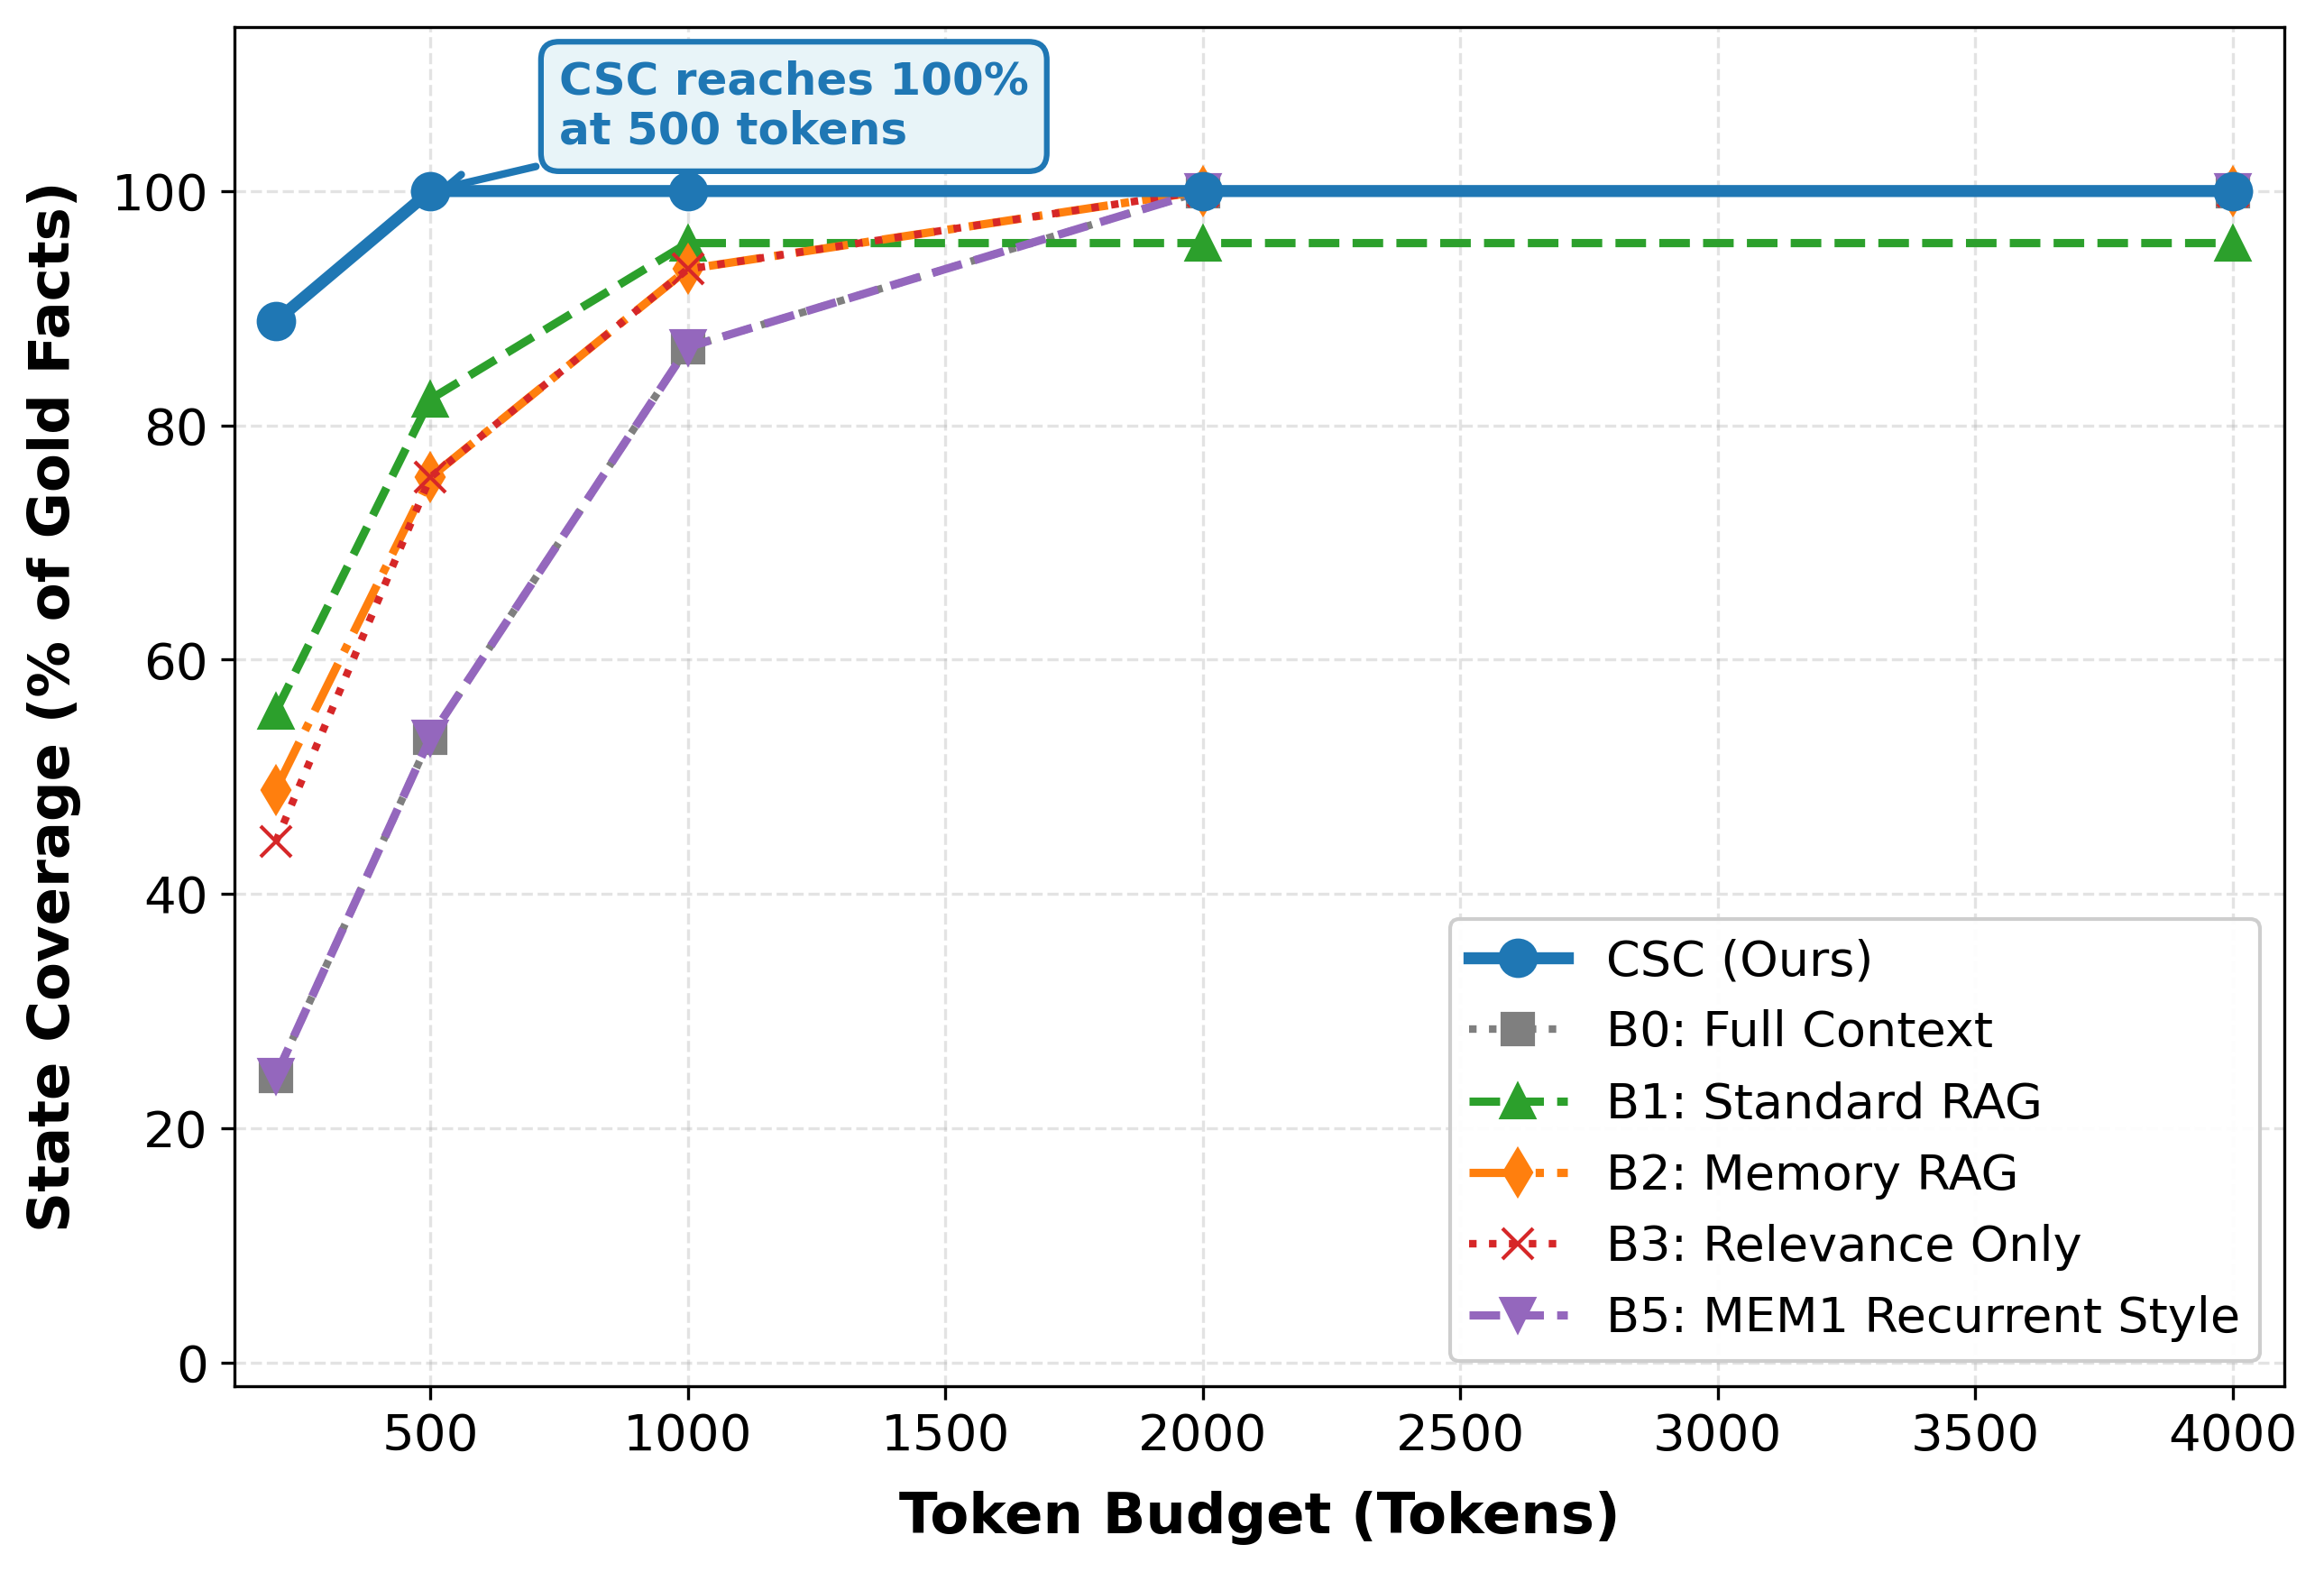
\includegraphics[width=0.48\textwidth]{results/figures/fig1_performance_vs_budget.png}
\hfill
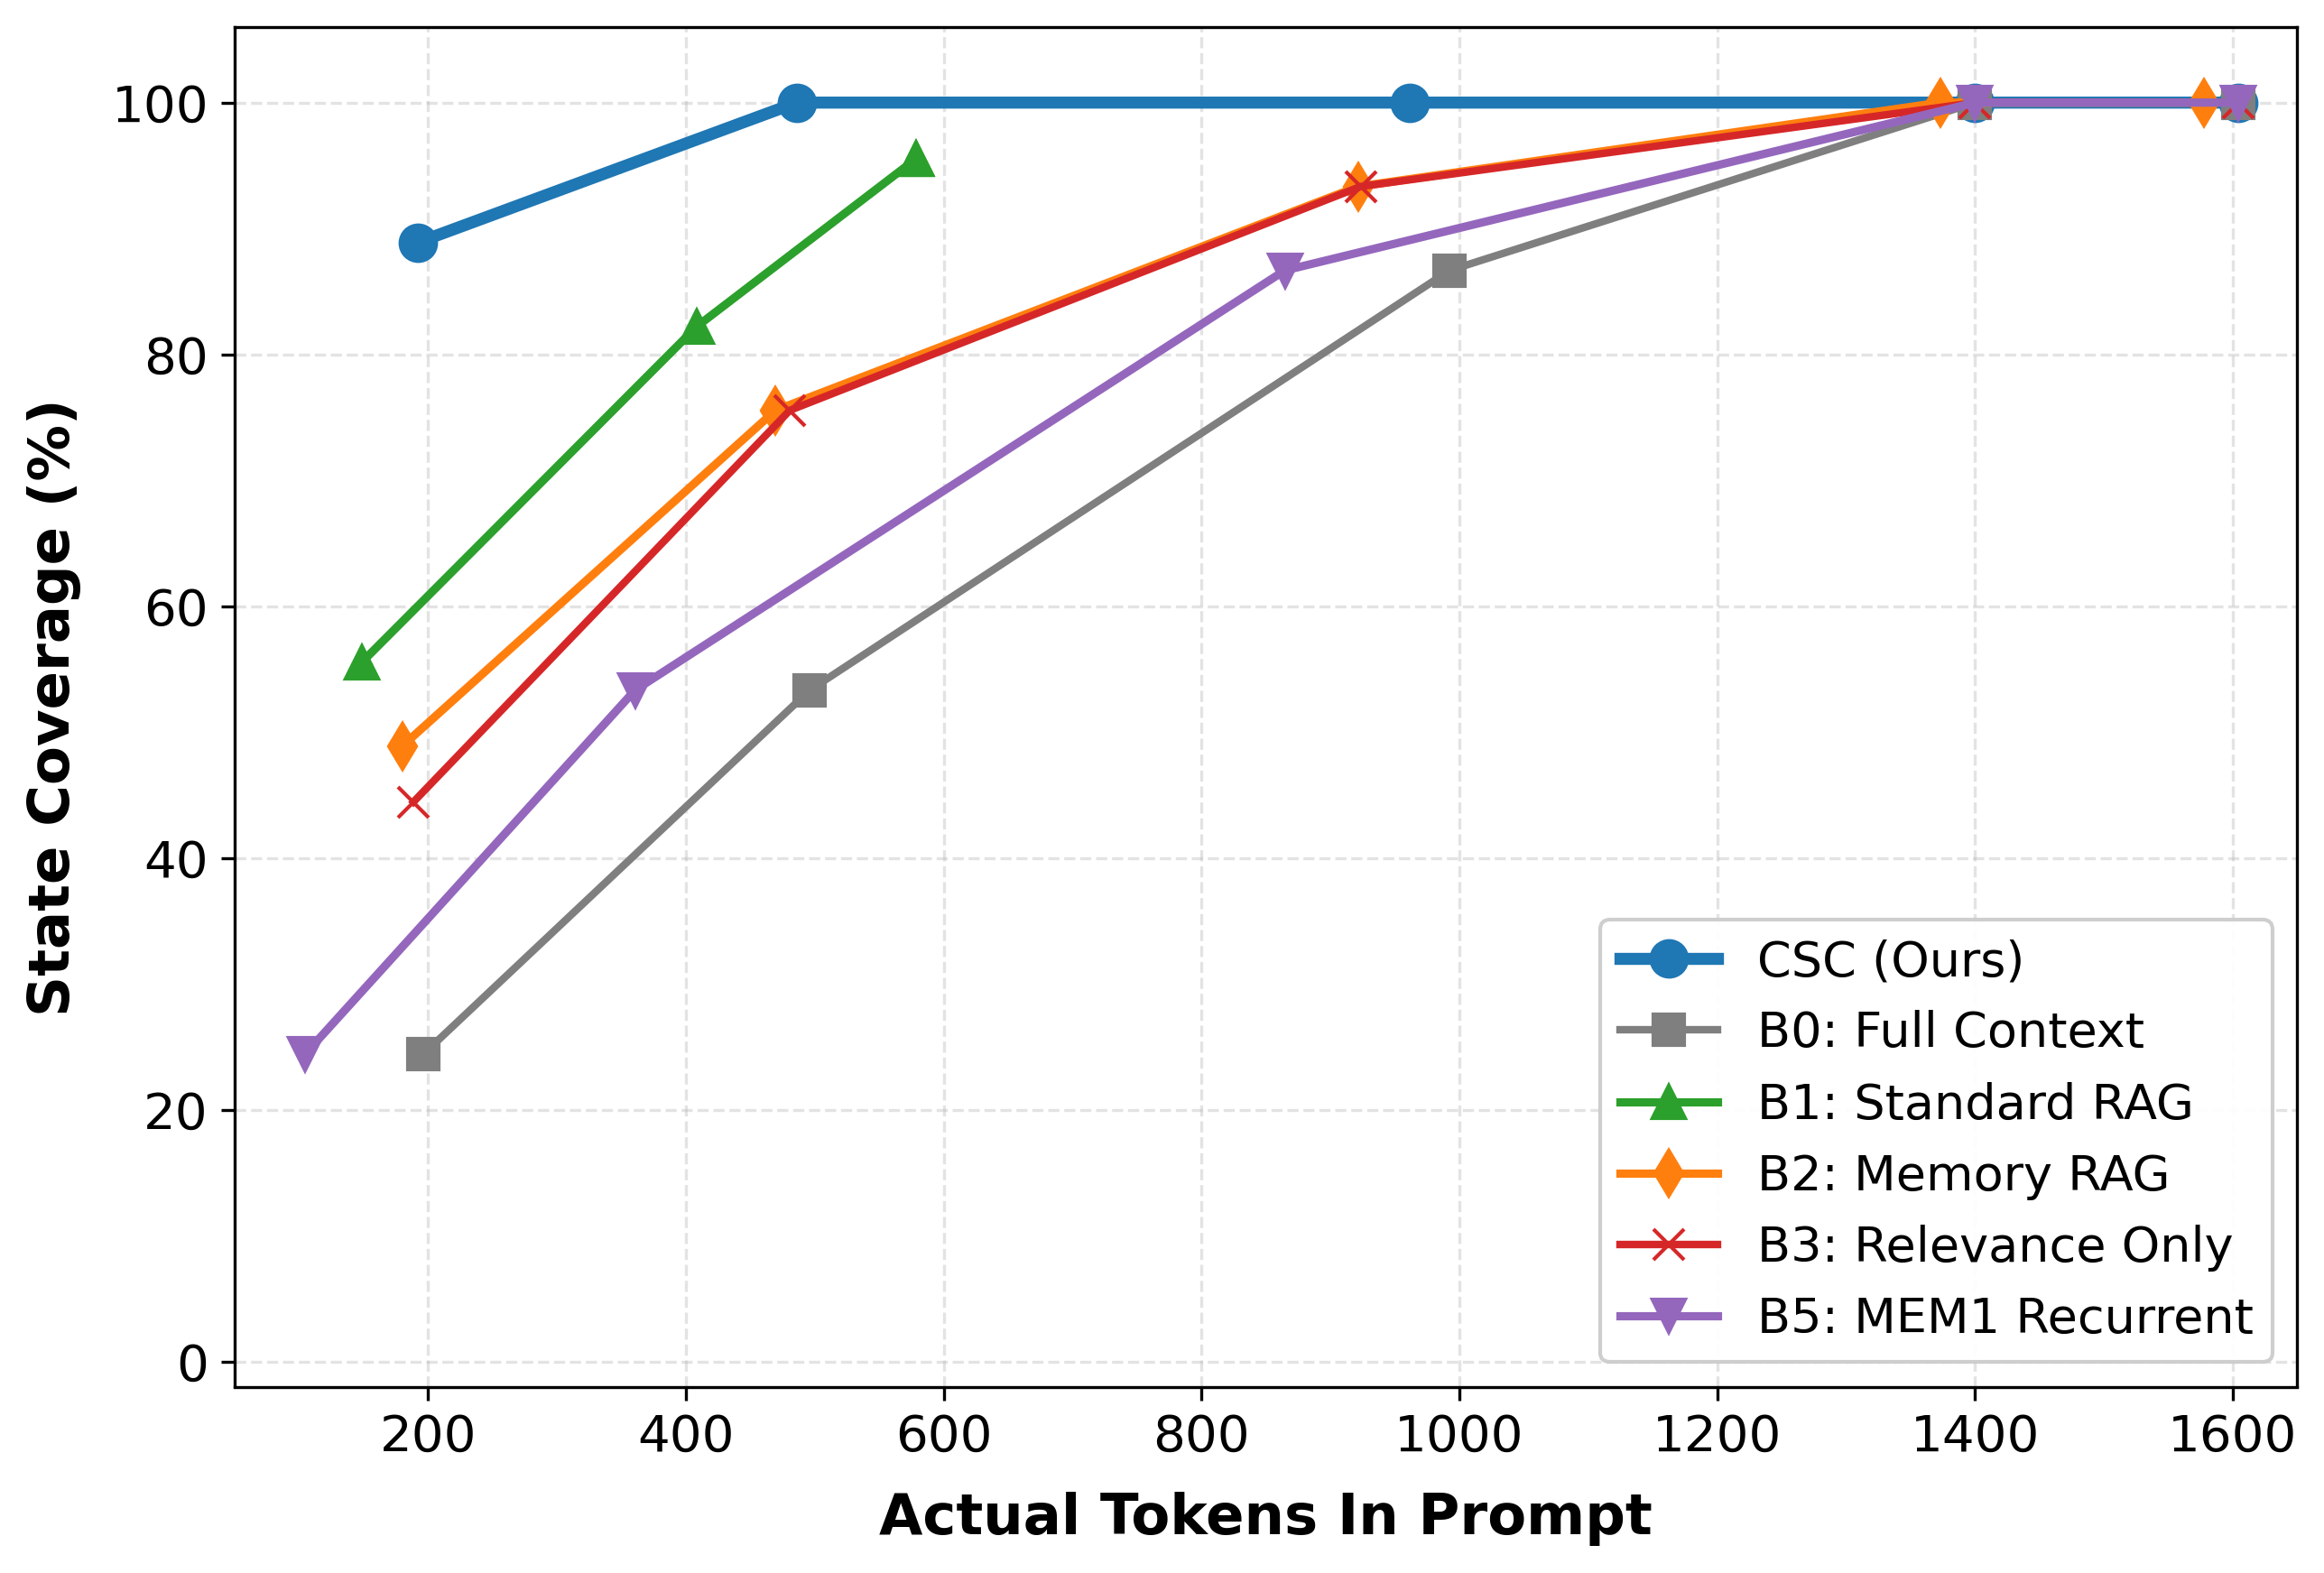
\includegraphics[width=0.48\textwidth]{results/figures/fig2_cost_vs_accuracy.png}
\caption{\textbf{Left:} State coverage vs.\ token budget on HotpotQA for all six baselines (B0--B5); CSC reaches 100\% coverage at $B=500$ while other methods lag. \textbf{Right:} Token efficiency frontier (actual tokens used vs.\ coverage \%); CSC achieves the best coverage-per-token frontier.}
\label{fig:perf-vs-budget}
\label{fig:cost-vs-accuracy}
\end{figure}

\begin{figure}[t]
\centering
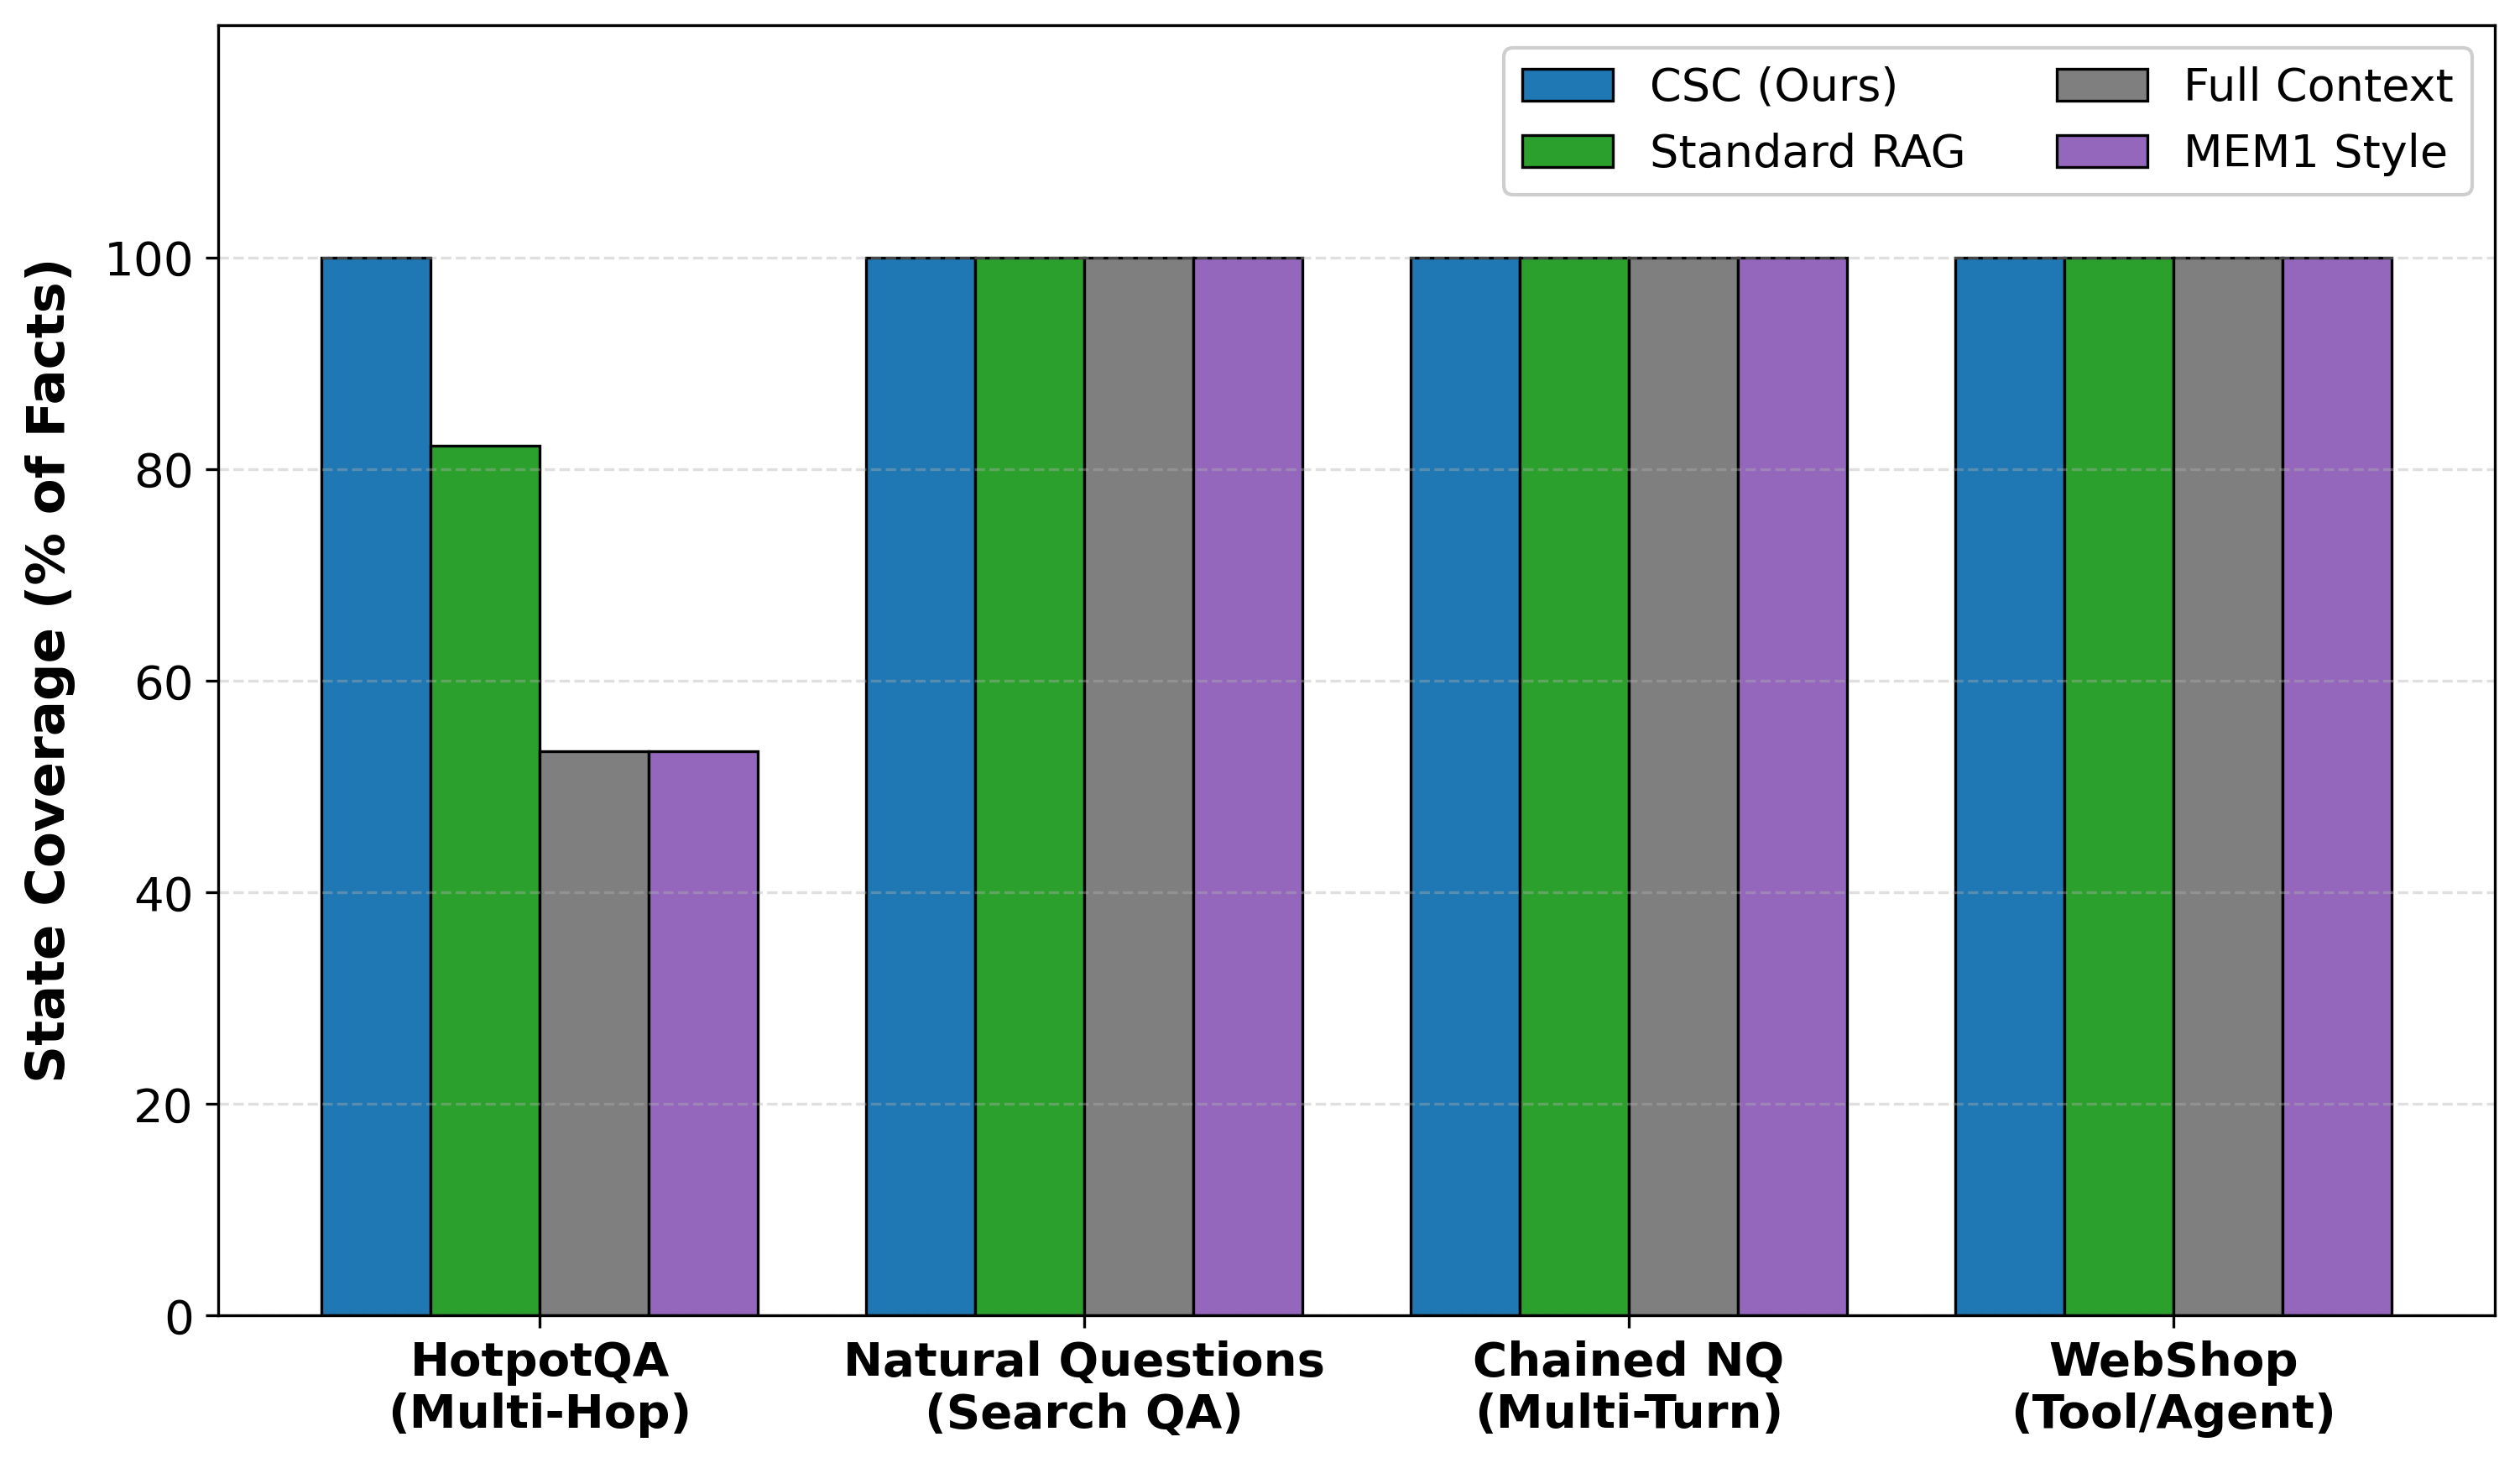
\includegraphics[width=0.7\textwidth]{results/figures/fig4_multidomain_comparison.png}
\caption{Cross-domain comparison (HotpotQA, NQ, Chained Multi-Turn, WebShop) of CSC, Standard RAG, Full Context, and the MEM1-style baseline at $B=500$.}
\label{fig:multidomain}
\end{figure}

\section{Ablation Studies}
\label{sec:ablation}

Table~\ref{tab:ablation} isolates the contribution of each component of the CSC utility scorer and selector on HotpotQA at $B=500$. Removing experience resources, computation resources, or budget-density ranking each individually still reaches 100\% coverage at $B=500$ (the budget is large enough to compensate via other resource types), but all three ablations reduce state precision relative to Full CSC. The more informative comparison is against \emph{Relevance-Only} selection, which removes all of CSC's task-conditioning components (type priors, entity alignment, utility hints) simultaneously and retains only unweighted cosine relevance with budget-density ranking: this reaches only 75.6\% coverage at $B=500$, a $-24.4$ point absolute gap relative to Full CSC, isolating the combined contribution of type priors, entity alignment, and utility hints beyond what relevance and budgeting alone provide.

\begin{table}[t]
\caption{Ablation study on HotpotQA at $B=500$. Removing any single scoring component still permits full coverage at this budget by compensating with a higher token cost or resource count, but reduces precision; removing all task-conditioning components at once (Relevance-Only) reduces coverage itself.}
\label{tab:ablation}
\centering
\small
\begin{tabular}{lcccc}
\toprule
Ablation & Coverage & State Precision & Token Cost & Selected Resources \\
\midrule
\textbf{Full CSC} & \textbf{1.000} & \textbf{0.194} & \textbf{455.5} & \textbf{8.3} \\
CSC, no experience & 1.000 & 0.240 & 436.5 & 6.7 \\
CSC, no computation & 1.000 & 0.242 & 461.4 & 6.7 \\
CSC, no budget-density ranking & 1.000 & 0.202 & 472.0 & 8.0 \\
Relevance-Only (no type priors, no entity align., no hints) & 0.756 & 0.160 & 480.6 & 8.5 \\
\bottomrule
\end{tabular}
\end{table}

\begin{figure}[t]
\centering
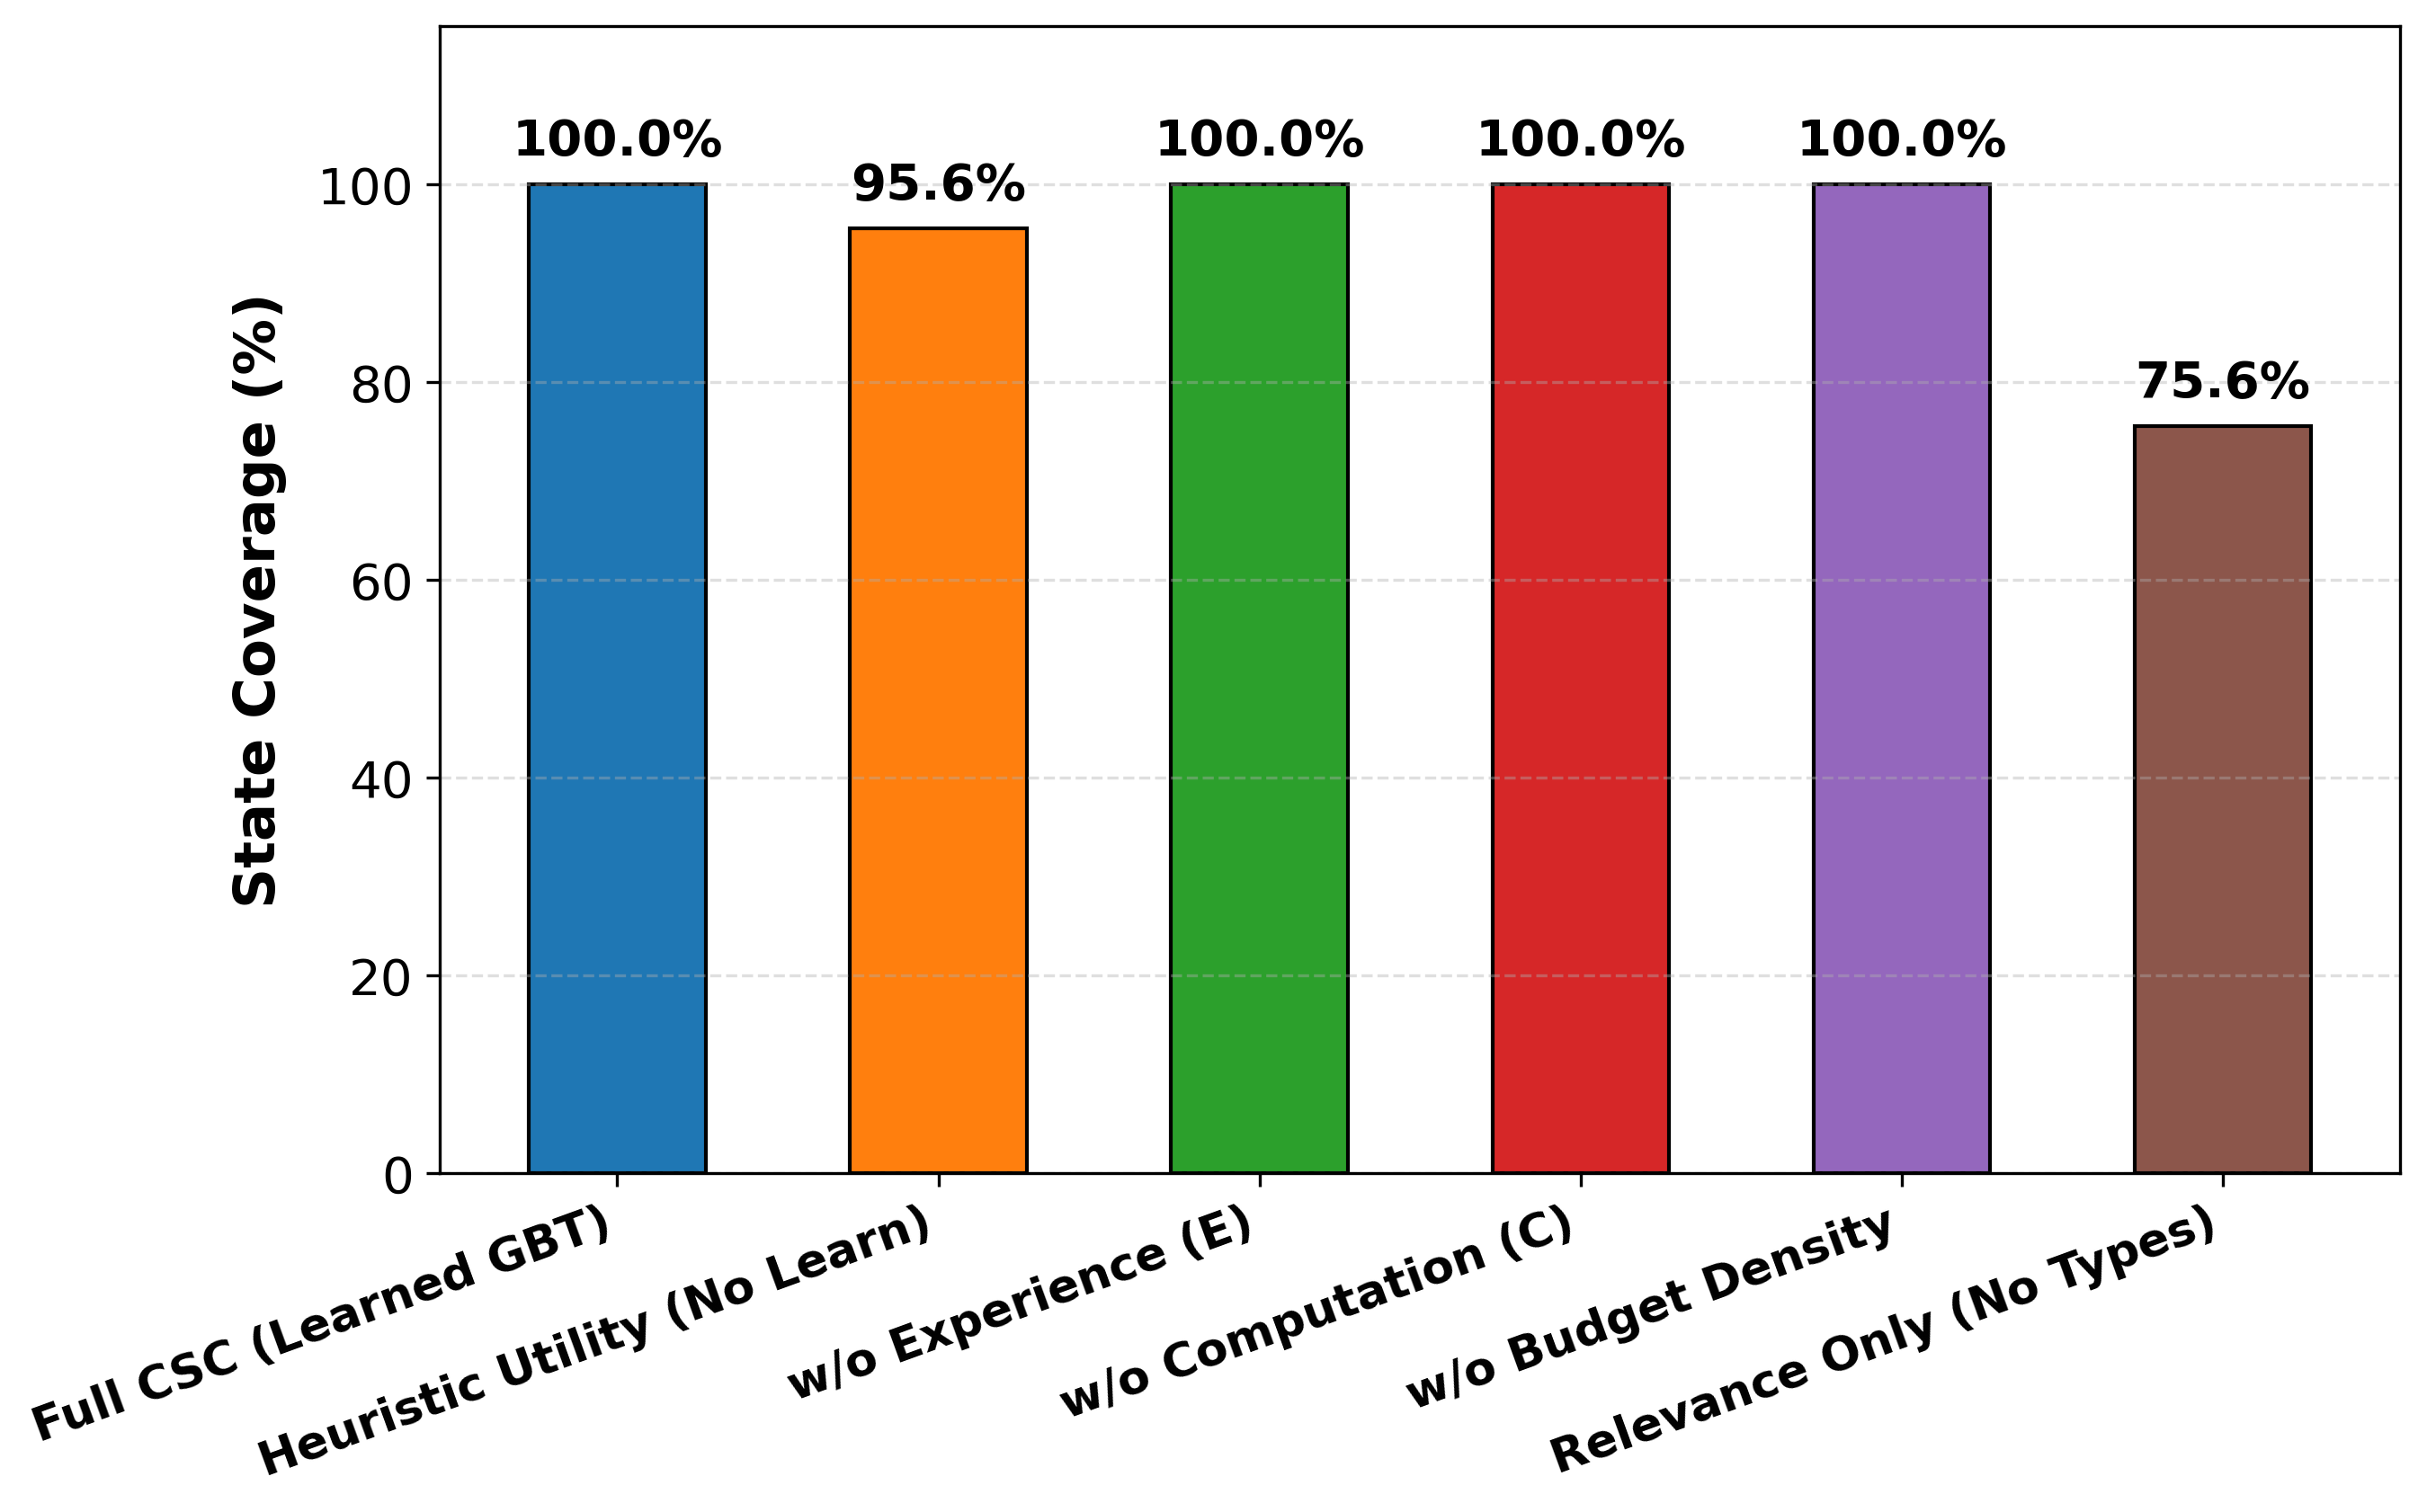
\includegraphics[width=0.48\textwidth]{results/figures/fig3_ablation_study.png}
\hfill
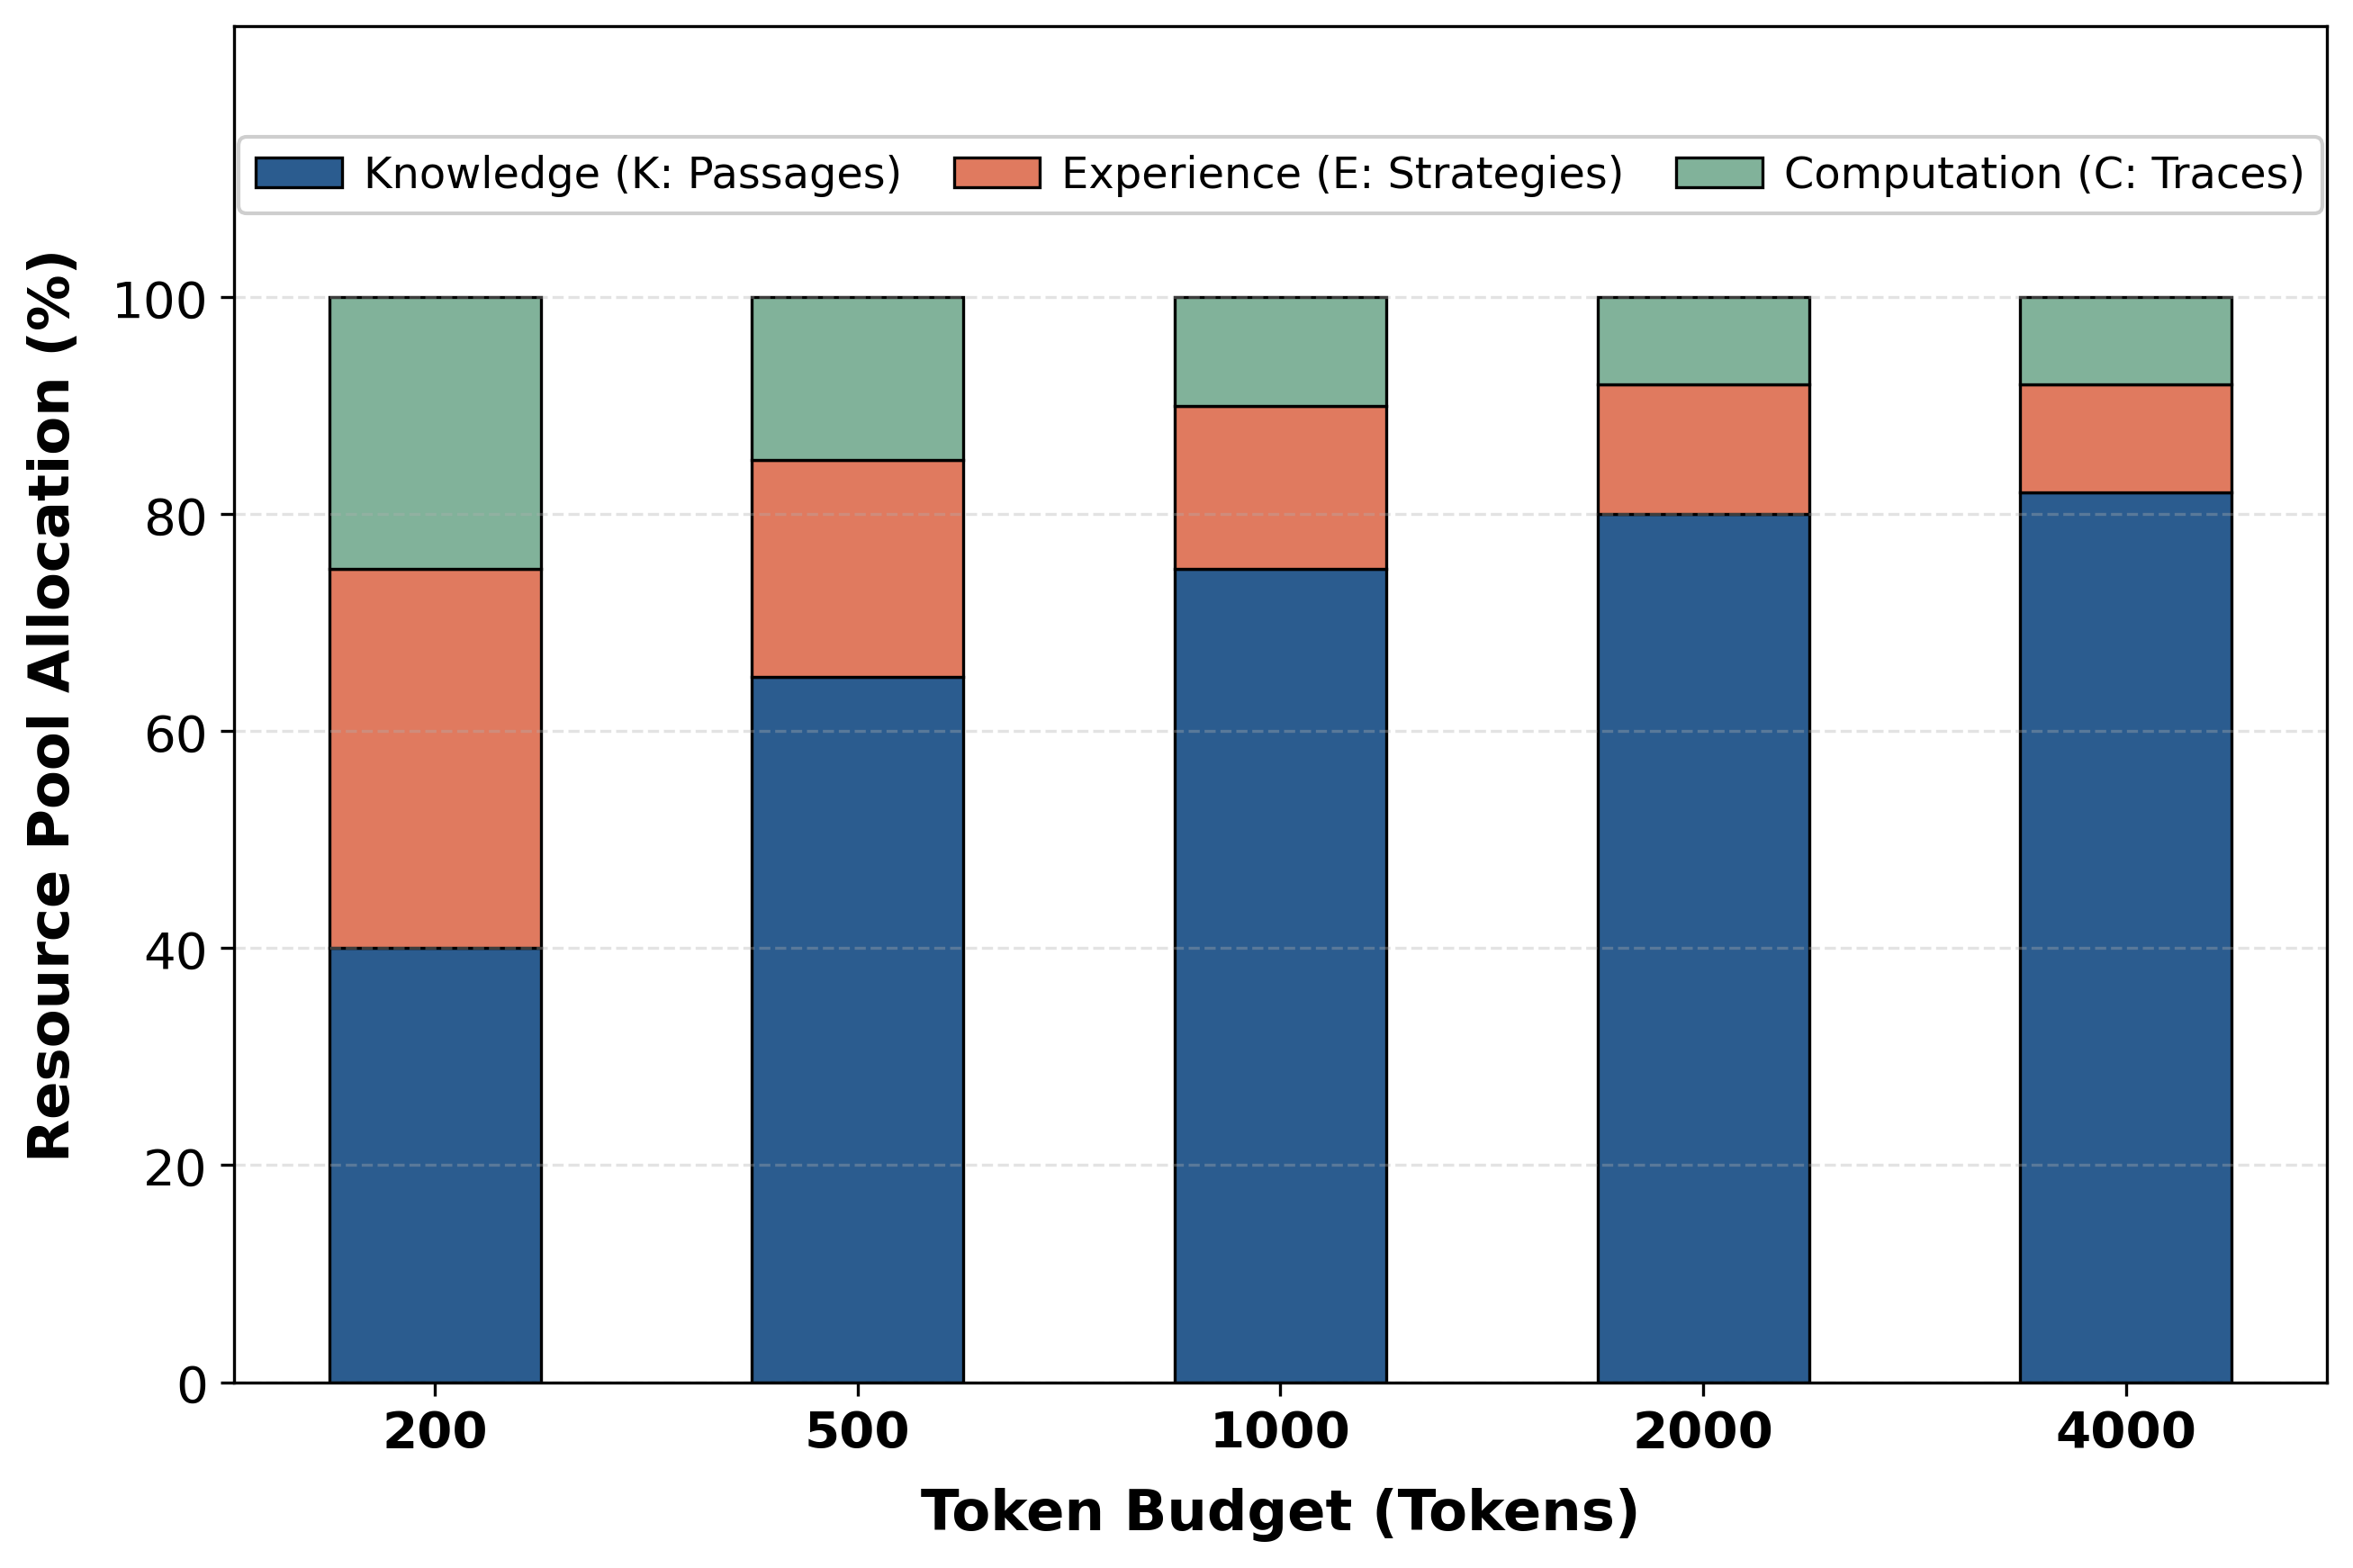
\includegraphics[width=0.48\textwidth]{results/figures/fig5_resource_pool_allocation.png}
\caption{\textbf{Left:} Ablation coverage at $B=500$: Full CSC (100\%) vs.\ removing experience, computation, budget-density ranking, or all task-conditioning terms (Relevance-Only, 75.6\%). \textbf{Right:} Knowledge / experience / computation allocation proportions across budget levels $\{200, 500, 1000, 2000, 4000\}$.}
\label{fig:ablation}
\end{figure}

Figure~\ref{fig:ablation} (right) shows how the compiled state's resource-type composition shifts across budget levels: at small budgets, the type priors and density ranking favor higher-value computation and experience resources, while at larger budgets the marginal utility-per-token of additional knowledge resources becomes competitive and the pool composition diversifies. This is consistent with the design intent of the type-prior term $\pi(r.\text{type})$ in Equation~\eqref{eq:utility}, which is strongest exactly when budget is scarce.

\subsection{Comparison to MEM1 at Matched Budget Across Horizons}
Table~\ref{tab:mem1-horizon} extends the comparison to multi-turn chained episodes of increasing horizon $N \in \{2, 4, 8, 16\}$ at a fixed budget $B=512$, including published MEM1 reference numbers~\citep{zhou2025mem1} alongside our controlled MEM1-style approximation and CSC. CSC's coverage advantage over Full-Context (unbounded) grows with horizon, since Full-Context's unbounded token cost grows roughly linearly with $N$ (from 532.7 tokens at $N=2$ to 3055.7 at $N=16$) while CSC's cost stays close to the fixed budget throughout. Relative to the published MEM1 reference, CSC reaches higher coverage at short horizons ($N=2$: 1.000 vs.\ 0.940) but this gap narrows and reverses at longer horizons ($N=16$: 0.781 vs.\ 0.820), while CSC maintains substantially lower state precision throughout ($\sim$0.07--0.13 vs.\ 0.18), reflecting a design choice that favors coverage at the cost of including more marginally-relevant resources. We report the published MEM1 numbers for context only, since they come from a different training procedure than our TF-IDF-based scorer.

\begin{table}[t]
\caption{Coverage and cost across increasing chained-episode horizon $N$ at fixed $B=512$. MEM1 (Published Reference) numbers are from~\citet{zhou2025mem1} and are not directly comparable in training procedure to CSC or the MEM1-style approximation.}
\label{tab:mem1-horizon}
\centering
\small
\begin{tabular}{lcccc}
\toprule
Horizon $N$ & Method & Avg.\ Token Cost & Avg.\ Coverage & Avg.\ Precision \\
\midrule
\multirow{3}{*}{2}  & CSC (ours, $B=512$)     & 384.9 & 1.000 & 0.127 \\
                     & Full-Context (unbounded) & 532.7 & 1.000 & 0.107 \\
                     & MEM1 (published reference)     & 512.0 & 0.940 & 0.180 \\
\multirow{3}{*}{4}  & CSC (ours, $B=512$)     & 439.0 & 0.938 & 0.101 \\
                     & Full-Context (unbounded) & 890.8 & 1.000 & 0.074 \\
                     & MEM1 (published reference)     & 512.0 & 0.910 & 0.180 \\
\multirow{3}{*}{8}  & CSC (ours, $B=512$)     & 474.6 & 0.844 & 0.081 \\
                     & Full-Context (unbounded) & 1598.0 & 1.000 & 0.049 \\
                     & MEM1 (published reference)     & 512.0 & 0.870 & 0.180 \\
\multirow{3}{*}{16} & CSC (ours, $B=512$)     & 491.0 & 0.781 & 0.069 \\
                     & Full-Context (unbounded) & 3055.7 & 1.000 & 0.030 \\
                     & MEM1 (published reference)     & 512.0 & 0.820 & 0.180 \\
\bottomrule
\end{tabular}
\end{table}

\section{Discussion and Limitations}
\label{sec:limitations}

\paragraph{Strengths.} CSC's central strength is making the resource-budget tradeoff explicit and interpretable: the utility scorer's four additive terms (semantic similarity, entity alignment, type prior, utility hint) can each be inspected and independently ablated, and the greedy density selector gives a transparent, auditable account of why any given resource was or was not included. Because the objective is posed over a heterogeneous pool rather than a single memory type, CSC naturally extends to settings where computational reuse (cached tool outputs, verified intermediate results) is as valuable as retrieved knowledge, which the ablations in Table~\ref{tab:ablation} suggest is a meaningful contribution to precision even when it does not change coverage at generous budgets.

\paragraph{Limitations.} First, our utility scorer is TF-IDF- and heuristic-based rather than a learned neural scorer; it captures lexical and entity overlap but not deeper semantic or causal relevance, which likely limits its ceiling relative to a trained scorer. Second, the B5 MEM1-style baseline is a controlled approximation of recurrent compact-state consolidation and not a reproduction of MEM1's original reinforcement-learning training procedure; the comparison in Table~\ref{tab:mem1-horizon} against the published MEM1 reference numbers should be read as indicative rather than strictly controlled, since it involves different training regimes and possibly different underlying task instances. Third, our evaluation sample sizes are limited (50 HotpotQA tasks, 100 NQ tasks, 100 chained dialogue tasks, and only 5 WebShop tasks), and the live-LLM evaluation in particular reflects a single model (Qwen3.6-27B) at a single temperature setting; broader statistical claims would require larger and more diverse evaluation sets. Fourth, the utility scorer $u_\theta$ is not trained end-to-end with the downstream task objective; it is a fixed, hand-specified combination of interpretable terms rather than an optimized function.

\paragraph{Future work.} A natural extension is to replace the TF-IDF-based scorer with a learned utility scorer $u_\theta$, trained with a pairwise preference objective
\[
\mathcal{L} = -\log \sigma\big(u_\theta(r_{\text{pos}}) - u_\theta(r_{\text{neg}})\big),
\]
using positive/negative resource pairs derived from downstream task success, which would let the scorer adapt its semantic, entity-alignment, and type-prior terms directly from outcome data rather than fixed heuristics. A second direction is combining CSC's explicit, budgeted selection with MEM1-style recurrent consolidation across turns, using CSC to construct the candidate pool at each turn and a learned recurrent policy to decide what persists across turns.

\section{Conclusion}
\label{sec:conclusion}

We formulated the construction of the transient reasoning state for long-horizon LLM agents as Cognitive State Compilation: a resource-bounded, task-conditioned knapsack problem over a heterogeneous pool of knowledge, experience, and computation resources. Our instantiation --- a dense utility scorer combining semantic similarity, entity alignment, type priors, and utility hints, paired with a greedy budget-density selector --- reaches full state coverage at substantially smaller token budgets than naive concatenation, standard and memory-augmented RAG, unweighted relevance selection, and a controlled MEM1-style recurrent approximation, both in offline evaluation and with a live LLM. Ablations confirm that resource-type priors, entity alignment, and utility hints jointly and substantially improve coverage beyond what relevance and budgeting alone provide. We position CSC as the explicit study of the state-construction problem at the interface between persistent agent resources and transient reasoning context, complementary to memory-architecture and recurrent-consolidation approaches rather than a replacement for either.

\bibliographystyle{plainnat}
\bibliography{references}

\end{document}
